\documentclass{article}
\usepackage[T1]{fontenc}
\usepackage[utf8]{inputenc}
\usepackage[a4paper, total={6in, 8in}]{geometry}
%\usepackage[icelandic]{babel}
\usepackage{graphicx} %package to manage images

\usepackage{hyperref}

\usepackage{xcolor}
\usepackage{listings}

\colorlet{mygray}{black!30}
\colorlet{mygreen}{green!60!blue}
\colorlet{mymauve}{red!60!blue}

\lstset{
  backgroundcolor=\color{gray!10},  
  basicstyle=\ttfamily,
  columns=fullflexible,
  breakatwhitespace=false,      
  breaklines=true,                
  captionpos=b,                    
  commentstyle=\color{mygreen}, 
  extendedchars=true,              
  frame=single,                   
  keepspaces=true,             
  keywordstyle=\color{blue},      
  language=c++,                 
  numbers=none,                
  numbersep=5pt,                   
  numberstyle=\tiny\color{blue}, 
  rulecolor=\color{mygray},        
  showspaces=false,               
  showtabs=false,                 
  stepnumber=5,                  
  stringstyle=\color{mymauve},    
  tabsize=3,                                     
  title=\lstname 
}

\title{Embedded Group Project}
\author{Steinarr Hrafn Höskuldsson\\
Arnþór Gíslason\\
Reykjavik University}
\date{September 2022}

\begin{document}

\maketitle

\section*{Part 1}
The hall effect sensor has 7 hole pairs and with each revolution of the motor shaft, the signal will cycle 7 times. With two signals, 90° out of phase there are 28 edges per revolution equally spaced. The maximum motor speed is rated at 15.000 RPM or 250 Hz. The minimum time between edges is thus expected to be \((28*250Hz)^{-1}) = 143 \mu s\)

An encoder class was written that polls pins 9 and 10 on the Arduino and keeps track of how many pulses have been registered. 

The two signals and the signal from the LED pin were wired to an RTB2004 oscilloscope and observed that we could turn the LED on for 120 microseconds without dropping pulses. This test did not include printing the encoder.position() to the serial port. 


\begin{figure}[h]
    \centering
    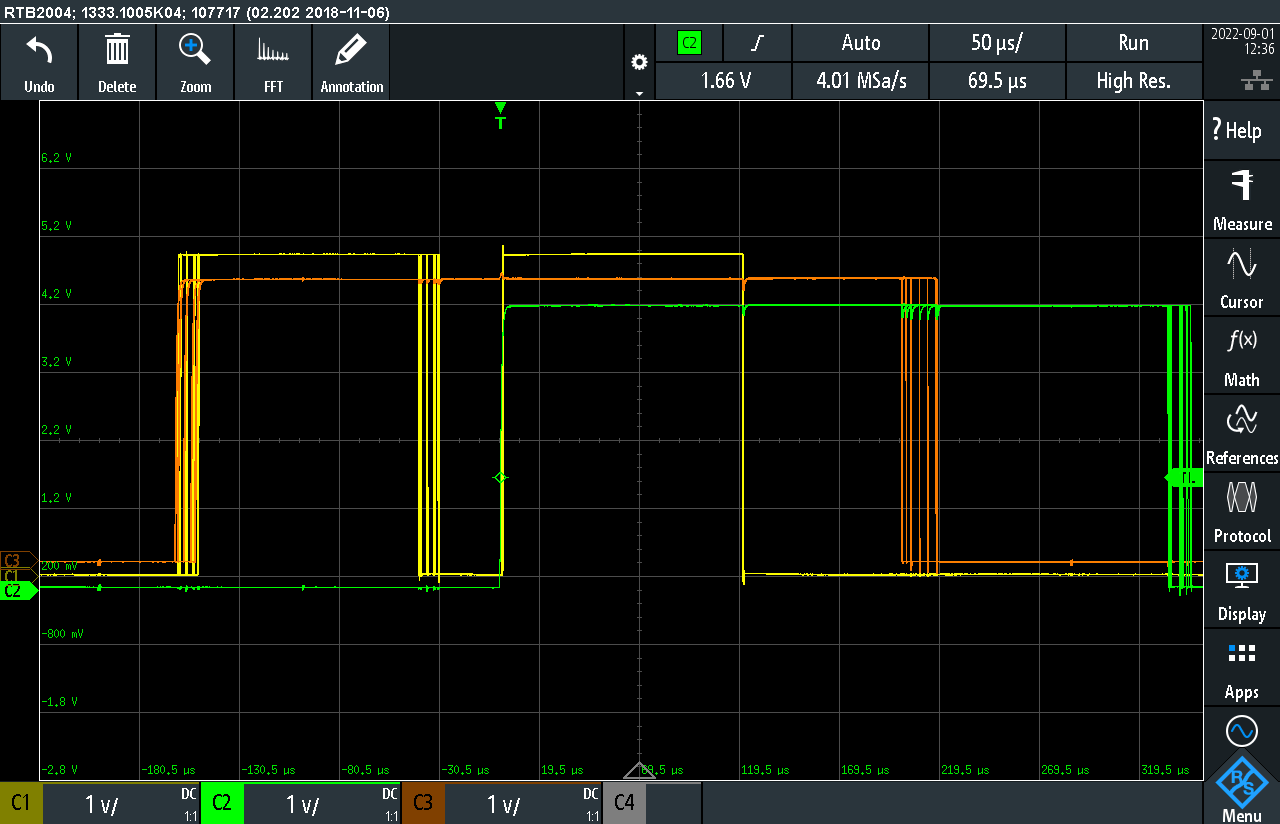
\includegraphics[width=0.75\textwidth]{Project1RotaryEncoder/oscilloscope_part1_120ms.PNG}
    \caption{Screenshot of the RTB2004 oscilloscope, LED (yellow) is turned on for 120 microsecond at pulse detection. Note that the graphs have been vertically shifted slightly to make them more visible.}
    \label{fig:osc120}
\end{figure}

With the motor running and the Arduino printing regularily to the serial port, a pin was toggled each time the monitor detected a state change. A jitter and a period of inactivity on the toggled pin was observed indicating that there were periods where the microcontroller was missing pulses while transmitting on the UART. The baud rate was set at 9600 baud which translates to about 1ms per character written and the microcontroller was transmitting up to 6 characters at a time. 


\begin{figure}[h]
    \centering
    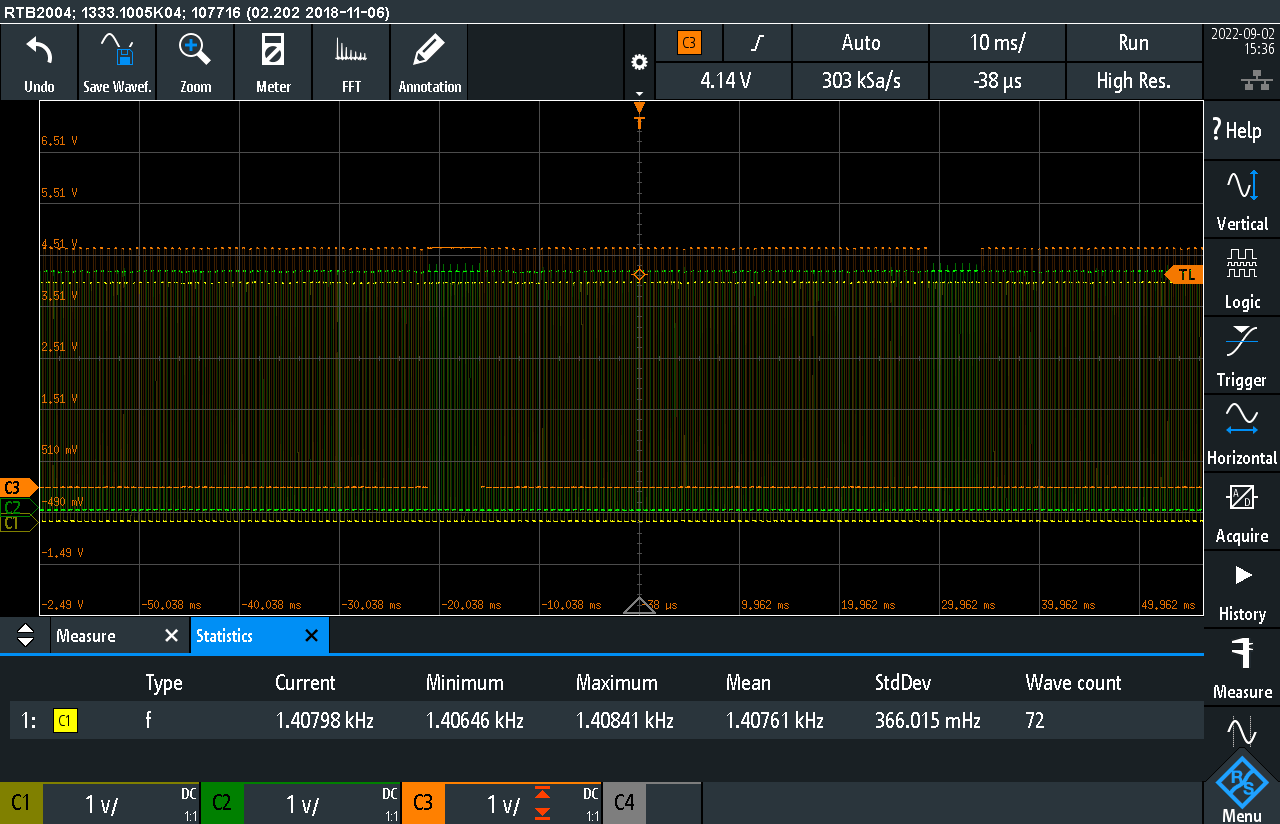
\includegraphics[width=0.75\textwidth]{Project1RotaryEncoder/oscilloscope_missing_pulses.PNG}[h!]
    \caption{While writing to the serial port, the Arduino is not polling the input pins, causing dropped pulses. This can be seen in the missing LED(orange) pulses}
    \label{fig:oscdrop}
\end{figure}


\section*{Part 2}
Using interrupts to monitor the pins allows us to count the pulses even while writing to the serial port.

After implementing interrupts neither jitter nor periods of inactivity were observed during run-time. Obviously, the interrupts were running during the delay which was waiting for the UART controller to transmit. 

For this exact problem, the baud rate may have been increased substantially causing the time to transmit the characters to be reduced below the minimum time before pulses. Alternatively, the wait for each character transmission could have been eliminated and the main loop made to check if the UART controller was able to receive a new character to transmit.


A video of the encoder working can be seen at:\newline  \url{https://youtube.com/shorts/oQev6f1VCDk}

repo: \newline\url{https://github.com/Steinarr134/EmbeddedGroupProjects/tree/main/Project1RotaryEncoder}
\newpage
\section*{Appendix}
\appendix
\section{Code}\label{appendix:code}

\lstinputlisting[caption=encoder\_simple.h]{Project1RotaryEncoder/src/encoder_simple.h}

\lstinputlisting[caption=timer\_msec.cpp]{Project1RotaryEncoder/src/encoder_simple.cpp}

\lstinputlisting[caption=main.cpp]{Project1RotaryEncoder/src/main.cpp}

\end{document}
